\section{异步推理机制设计与理论分析}\label{sec:async-inference}

\subsection{设计思路}\label{sec:async-inf-motivation}

回到 4.1 节提出的问题：在同步流水线下，每完成一次模型推理后，
系统还要顺序执行整段动作块，这意味着推理时间和动作执行时间被直接相加，
有效 FPS 只能由两者的总耗时决定，在本平台上约为 19 FPS。
如果能把下一次推理重叠到当前动作块的执行阶段内，
就有机会把系统吞吐恢复到更接近目标控制频率的水平。这就是推理异步化的核心设计动机。
Real-Time Chunking\cite{realtimechunking} 工作同样指出，对于输出 action chunk 的策略，
可以采用“执行当前 chunk 的同时生成下一段动作”的方式，
以降低高延迟策略模型对实时控制频率的影响。

与舵机读写不同的是：推理过程纯粹是 Python+PyTorch
计算，不与任何半双工硬件资源耦合，理论上具备真正并行的物理基础；
LeRobot 上游也已为此提供了完整的双进程实现\cite{smolvla}，无需自行从零开发。
因此本节的工作不再是“评估能不能做”，而是“评估在树莓派 5 + 当前 ACT 模型
的具体参数下，做了能不能带来实际收益”。

\subsection{实现结构}\label{sec:async-inf-arch}

图~\ref{fig:async-inf-arch}展示了异步推理架构：
Robot Client 与 Policy Server 是两个独立进程。
前者负责硬件连接、观测阶段、控制循环与动作执行，
后者负责加载模型、完成推理并返回动作序列；
二者通过 gRPC 交换带时间戳和步号的观测与动作序列。

\begin{figure}[htbp]
  \centering
  \begingroup
\definecolor{asyncClientFill}{HTML}{EEF8F0}
\definecolor{asyncClientStroke}{HTML}{2F855A}
\definecolor{asyncClientText}{HTML}{22543D}
\definecolor{asyncServerFill}{HTML}{EEF5FF}
\definecolor{asyncServerStroke}{HTML}{2B6CB0}
\definecolor{asyncServerText}{HTML}{1A365D}
\definecolor{asyncDarkText}{HTML}{1F2937}
\definecolor{asyncMutedText}{HTML}{4B5563}
\definecolor{asyncLine}{HTML}{4B5563}
\definecolor{asyncGray}{HTML}{9CA3AF}
\definecolor{asyncFooter}{HTML}{6B7280}
\resizebox{0.92\textwidth}{!}{%
\begin{tikzpicture}[
  x=1pt,
  y=-1pt,
  >=Triangle,
  process/.style={
    rounded corners=12pt,
    line width=3pt,
  },
  comm/.style={
    draw=asyncLine,
    line width=3pt,
    -{Triangle[length=16pt,width=18pt]},
  },
  pill/.style={
    rounded corners=25pt,
    draw=asyncGray,
    line width=1.5pt,
    fill=white,
  },
]
  \path[use as bounding box] (0,0) rectangle (1100,520);
  \fill[white] (0,0) rectangle (1100,520);

  \draw[process, fill=asyncClientFill, draw=asyncClientStroke]
    (70,72) rectangle (430,422);
  \node[
    font=\sffamily\bfseries\fontsize{34}{41}\selectfont,
    text=asyncClientText,
  ] at (250,135) {Robot Client 进程};
  \draw[asyncClientStroke!35, line width=2pt] (106,174) -- (394,174);

  \foreach \y/\txt in {
    222/{连接相机与舵机},
    272/{采集并发送观测},
    322/{维护控制循环与动作队列},
    372/{执行动作、对齐返回结果}
  } {
    \fill[asyncClientStroke!90] (104,\y-8) circle[radius=5pt];
    \node[
      anchor=west,
      font=\sffamily\fontsize{27}{34}\selectfont,
      text=asyncDarkText,
    ] at (125,\y) {\txt};
  }

  \draw[process, fill=asyncServerFill, draw=asyncServerStroke]
    (670,72) rectangle (1030,422);
  \node[
    font=\sffamily\bfseries\fontsize{34}{41}\selectfont,
    text=asyncServerText,
  ] at (850,135) {Policy Server 进程};
  \draw[asyncServerStroke!35, line width=2pt] (706,174) -- (994,174);

  \foreach \y/\txt in {
    242/{加载模型},
    302/{完成推理},
    362/{返回动作序列}
  } {
    \fill[asyncServerStroke!90] (704,\y-8) circle[radius=5pt];
    \node[
      anchor=west,
      font=\sffamily\fontsize{29}{36}\selectfont,
      text=asyncDarkText,
    ] at (725,\y) {\txt};
  }

  \draw[comm] (670,220) .. controls (620,220) and (480,220) .. (430,220);
  \draw[pill] (440,130) rectangle (660,204);
  \node[
    font=\sffamily\bfseries\fontsize{23}{28}\selectfont,
    text=asyncDarkText,
  ] at (550,156) {动作序列};
  \node[
    font=\sffamily\bfseries\fontsize{21}{26}\selectfont,
    text=asyncMutedText,
  ] at (550,187) {Action Chunk};

  \draw[comm] (430,292) .. controls (480,292) and (620,292) .. (670,292);
  \draw[pill] (440,304) rectangle (660,378);
  \node[
    font=\sffamily\bfseries\fontsize{23}{28}\selectfont,
    text=asyncDarkText,
  ] at (550,330) {观测结果};
  \node[
    font=\sffamily\bfseries\fontsize{21}{26}\selectfont,
    text=asyncMutedText,
  ] at (550,361) {Observation Result};

  \node[
    font=\sffamily\bfseries\fontsize{23}{30}\selectfont,
    text=asyncFooter,
  ] at (550,468) {gRPC 通信：Robot Client 发送观测，Policy Server 返回动作序列};
\end{tikzpicture}%
}
\endgroup

  \caption{异步推理架构}
  \label{fig:async-inf-arch}
\end{figure}

其中，控制端进程负责连接相机和舵机、维持控制循环，并将当前观测发送给
推理服务进程；
推理服务进程负责加载 ACT 模型，在收到观测后完成一次动作序列预测，
再将结果返回给控制端进程。这样，动作执行仍由本地控制循环逐帧推进，
而下一段动作的生成可以在另一进程中提前进行。

跨进程传输的数据对象包含时间戳和步号两个关键信息。
前者用于衡量观测发送、推理计算和动作返回之间的总时延，
后者用于判断一段动作序列对应的是哪一时刻的控制状态，
从而在异步回包到达时完成帧级对齐。

在控制端进程内部，主线程持续执行控制循环，
后台接收线程则专门等待推理服务进程返回结果。
二者通过一个带互斥保护的动作队列共享数据。
控制循环一方面从队列头部取出当前应执行的动作，另一方面持续监测队列剩余长度，
以决定何时触发下一次推理请求。与此同时，系统还维护最近一次已执行动作的步号、
当前 chunk\_size 以及队列是否即将耗尽等状态，用于支持后续的触发、对齐和兜底逻辑。

基于上述结构，异步推理的运行机制可以归纳为三个动作队列上的规则。
第一是提前触发：
控制端进程不会等当前动作块完全耗尽后再请求下一次推理，
而是在剩余动作下降到一定比例时提前发出新观测。
LeRobot 默认将这一比例设为 0.5，即动作块尚余一半时就启动下一次推理。
这样做的目的，是让新动作块尽可能在旧动作块执行完之前返回，从而把推理时间隐藏在执行阶段内部。

第二是时序对齐与融合：
新动作块返回后，控制端进程不会简单覆盖旧队列，
而是依据步号与当前执行位置进行对齐。
已经过时的动作会被直接丢弃，尚未执行但与旧动作块覆盖到同一未来时刻的部分则进行融合，
只把最终有效的未来动作重新写入队列。这样可以缓解动作块切换时的突变，
也是 temporal ensemble 在异步控制场景中的具体落地方式。

第三是空队列兜底：
若推理速度不足，导致动作队列接近耗尽，控制端进程会附带发送一个强制触发标记，
要求推理服务进程立即处理当前观测，而不再等待常规去重或合并逻辑。
这条路径本质上是异常兜底，用来避免队列彻底清空后控制循环停顿。
因此，强制触发出现得越频繁，越说明当前异步流水线离稳定工作区越远，
它也就成为后续实验中判断系统健康度的重要观测量。

\subsection{可行性不等式与异步推理触发阈值}\label{sec:async-inf-inequality}

异步推理的稳态行为受四个参数控制：chunk\_size $N$、
单次推理耗时 $T_{\text{infer}}$、目标执行频率 $F$、
以及异步推理触发阈值 $h$（实验中记为 hold）。
在 LeRobot 当前实现中，触发条件为
动作队列剩余比例不高于 $h$，
因此 $h$ 越大，触发越早；$h$ 越小，触发越晚。

为便于把推理耗时与动作队列长度放在同一尺度下比较，
这里引入 $D$ 表示一次推理返回前，主控制循环按目标频率大约会消耗掉的动作帧数。
换言之，$D$ 是推理时延折算到控制帧尺度后的结果，如式（\ref{eq:async-consumed-frames}）所示：
\begin{equation}
  D = T_{\text{infer}}F.
  \label{eq:async-consumed-frames}
\end{equation}
严格来说，调度条件中应使用从观测被 server 取走到动作 chunk
并入 client 队列的端到端返回时延；下文用 server 端记录的
$T_{\text{infer}}$ 近似这一时延，网络、序列化和队列调度开销则交由
4.3 节的实测结果反映。为简化推导，以下也忽略
动作步号不大于已执行步号带来的 1 帧端点差异。

代码中存在两个不同层次的约束。第一，触发必须足够早：
当队列剩余 $hN$ 帧时发出观测，如果 $D>hN$，
新动作在当前队列耗尽前无法返回，控制循环必然出现 stall。
因此触发条件可写为式（\ref{eq:async-trigger-condition}）：
\begin{equation}
  D \leq hN
  \quad\Longleftrightarrow\quad
  h \geq \frac{T_{\text{infer}}F}{N}.
  \label{eq:async-trigger-condition}
\end{equation}
这只是“本次请求来得及赶上当前队列”的条件。

第二，新 chunk 到货后并不会完整进入队列。
推理服务进程返回的动作步号从观测步号开始递增，
而控制端进程会丢弃所有动作步号不大于已执行步号的动作。
若返回前没有 stall，推理期间已经执行了约 $D$ 帧，
因此这里用 $N_{\text{eff}}$ 表示新 chunk 返回后，
剔除过期动作后真正能进入未来队列的有效帧数，
其近似值如式（\ref{eq:async-effective-chunk}）所示：
\begin{equation}
  N_{\text{eff}} \approx N - D = N - T_{\text{infer}}F.
  \label{eq:async-effective-chunk}
\end{equation}
由于同一 server 一次只能处理一个推理请求，下一轮推理仍要消耗约 $D$ 帧；
所以稳态不 stall 还需要满足式（\ref{eq:async-steady-condition}）：
\begin{equation}
  N_{\text{eff}} \geq D
  \quad\Longleftrightarrow\quad
  N \geq 2T_{\text{infer}}F.
  \label{eq:async-steady-condition}
\end{equation}

综合两者，异步流水线稳定无 stall 的近似条件应写为式（\ref{eq:async-stability-condition}）：
\begin{equation}
  \boxed{\,T_{\text{infer}}F \leq \min(hN,\; N/2)\,}.
  \label{eq:async-stability-condition}
\end{equation}
当 $h=0.5$ 时，两个约束同时退化为 $N \geq 2T_{\text{infer}}F$。
当 $h<0.5$ 时，主要风险是触发太晚；当 $h>0.5$ 时，
更早触发可以增加当前队列的等待余量，但不能突破
“一个 chunk 至少覆盖两个推理窗口”这一由 $N/2$ 决定的稳态上限。
因此在树莓派 5 这种推理慢、执行帧率固定的平台上，
$h$ 仍需作为调度参数单独扫描，但它不能替代对 $T_{\text{infer}}$ 或 $N$ 的优化。

为直观展示该不等式的物理含义，图~\ref{fig:async-case-a}--\ref{fig:async-inf-three-cases}
给出 $N=100$、$F=30$ 时三种代表性 $T_{\text{infer}}$ 取值下的稳态流水线时间线。
图中横轴为帧号（@30 FPS），纵向依次展示执行进程、推理进程与 chunk 队列内容；
蓝色块为正常执行帧，黄色块为 Temporal Ensemble 重叠区，红色块为 stall 停顿。

情况 A 对应 $T_{\text{infer}}=30$ 帧（1 s），此时 $D=30 \leq \min(hN,N/2)=50$，
不等式严格满足。推理进程在旧 chunk 执行至第 50 帧时启动，于第 80 帧前已完成，
形成约 20 帧宽的 Temporal Ensemble 重叠窗口，新旧 chunk 对这批帧均有预测，
融合后入队，执行全程连续无中断，稳态可达 30 FPS。

情况 B 对应 $T_{\text{infer}}=50$ 帧（1.67 s），此时 $D=50 = \min(hN,N/2)$，
恰好处于临界点。新 chunk 在旧 chunk 最后一帧执行完毕时精确到达，
既无 Temporal Ensemble 余量，也无 stall；但对参数扰动几乎没有容错空间，
推理轻微抖动即触发 stall。

情况 C 对应 $T_{\text{infer}}=70$ 帧（2.33 s），此时 $D=70 > \min(hN,N/2)=50$，
不等式不满足，出现周期性 stall。旧 chunk 耗尽后新 chunk 仍在推理中，
每周期产生约 20 帧 stall；stall 期间最新已执行动作步号冻结在第 99 帧，
新 chunk 过期帧为 $[50,99]$ 共 50 帧（非物理意义上的 70 帧），
有效帧 $[100,149]$ 共 50 帧进入队列，稳态有效 FPS $\approx 50/2.33 = 21.4$。

\begin{figure}[htbp]
  \centering
  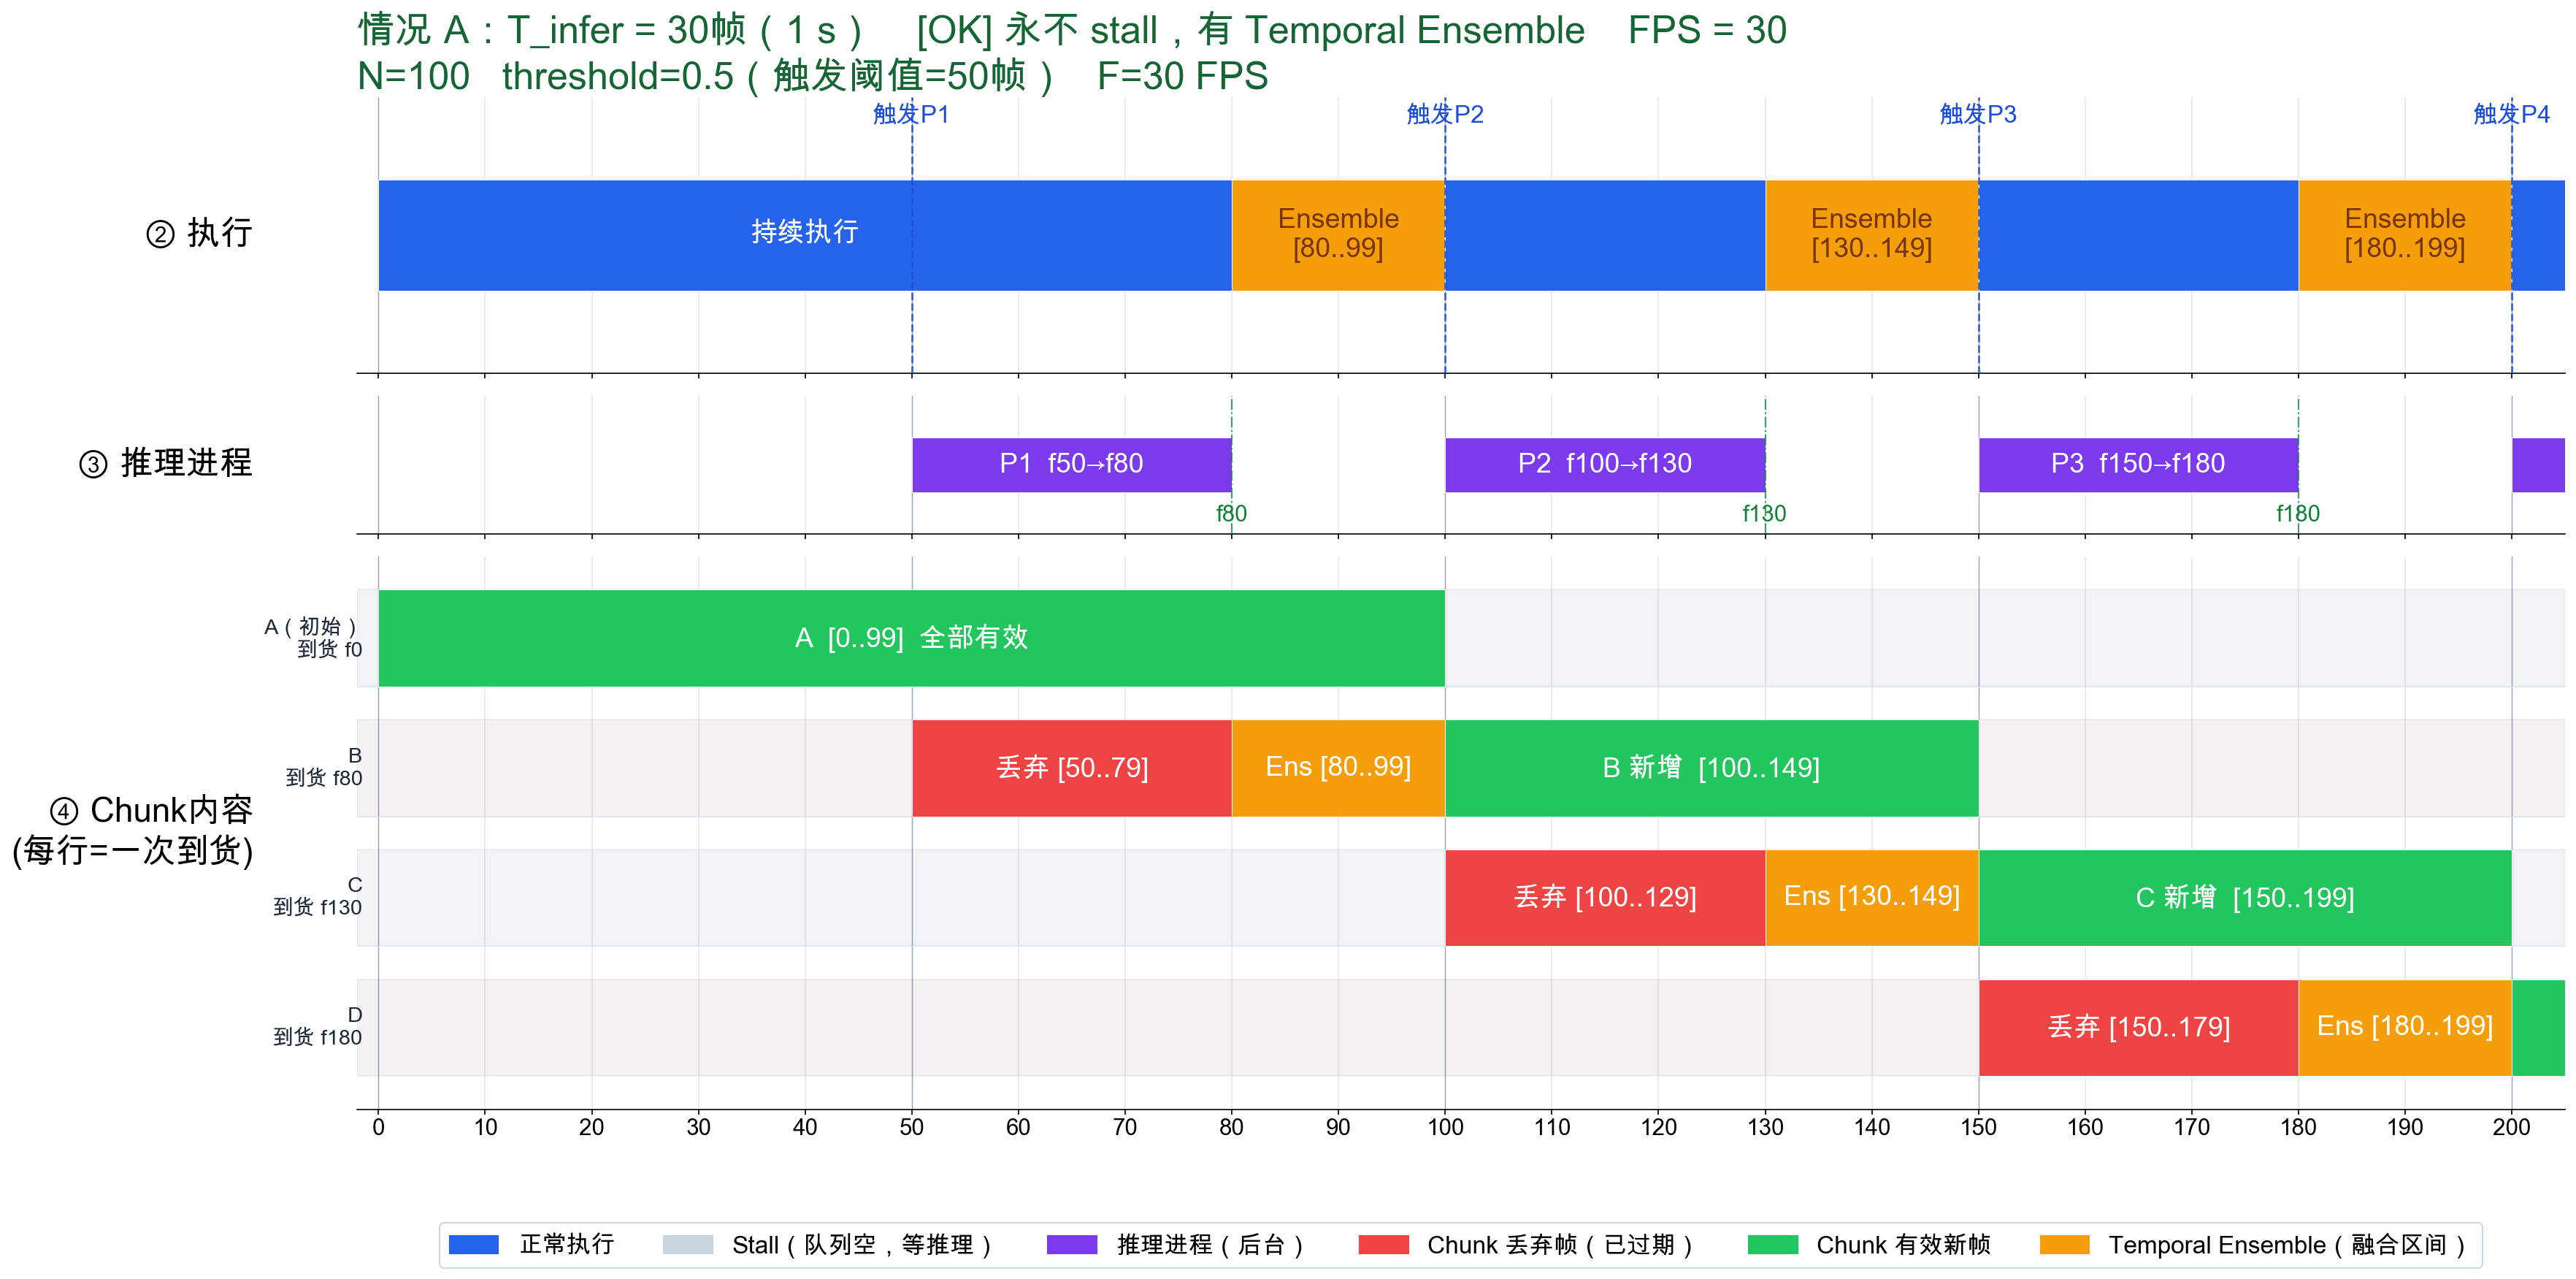
\includegraphics[width=\linewidth]{4_优化/images/async_inference_A.png}
  \caption{情况 A：$T_{\text{infer}}=30$ 帧，不等式满足，稳态 30 FPS}
  \label{fig:async-case-a}
\end{figure}

\begin{figure}[htbp]
  \centering
  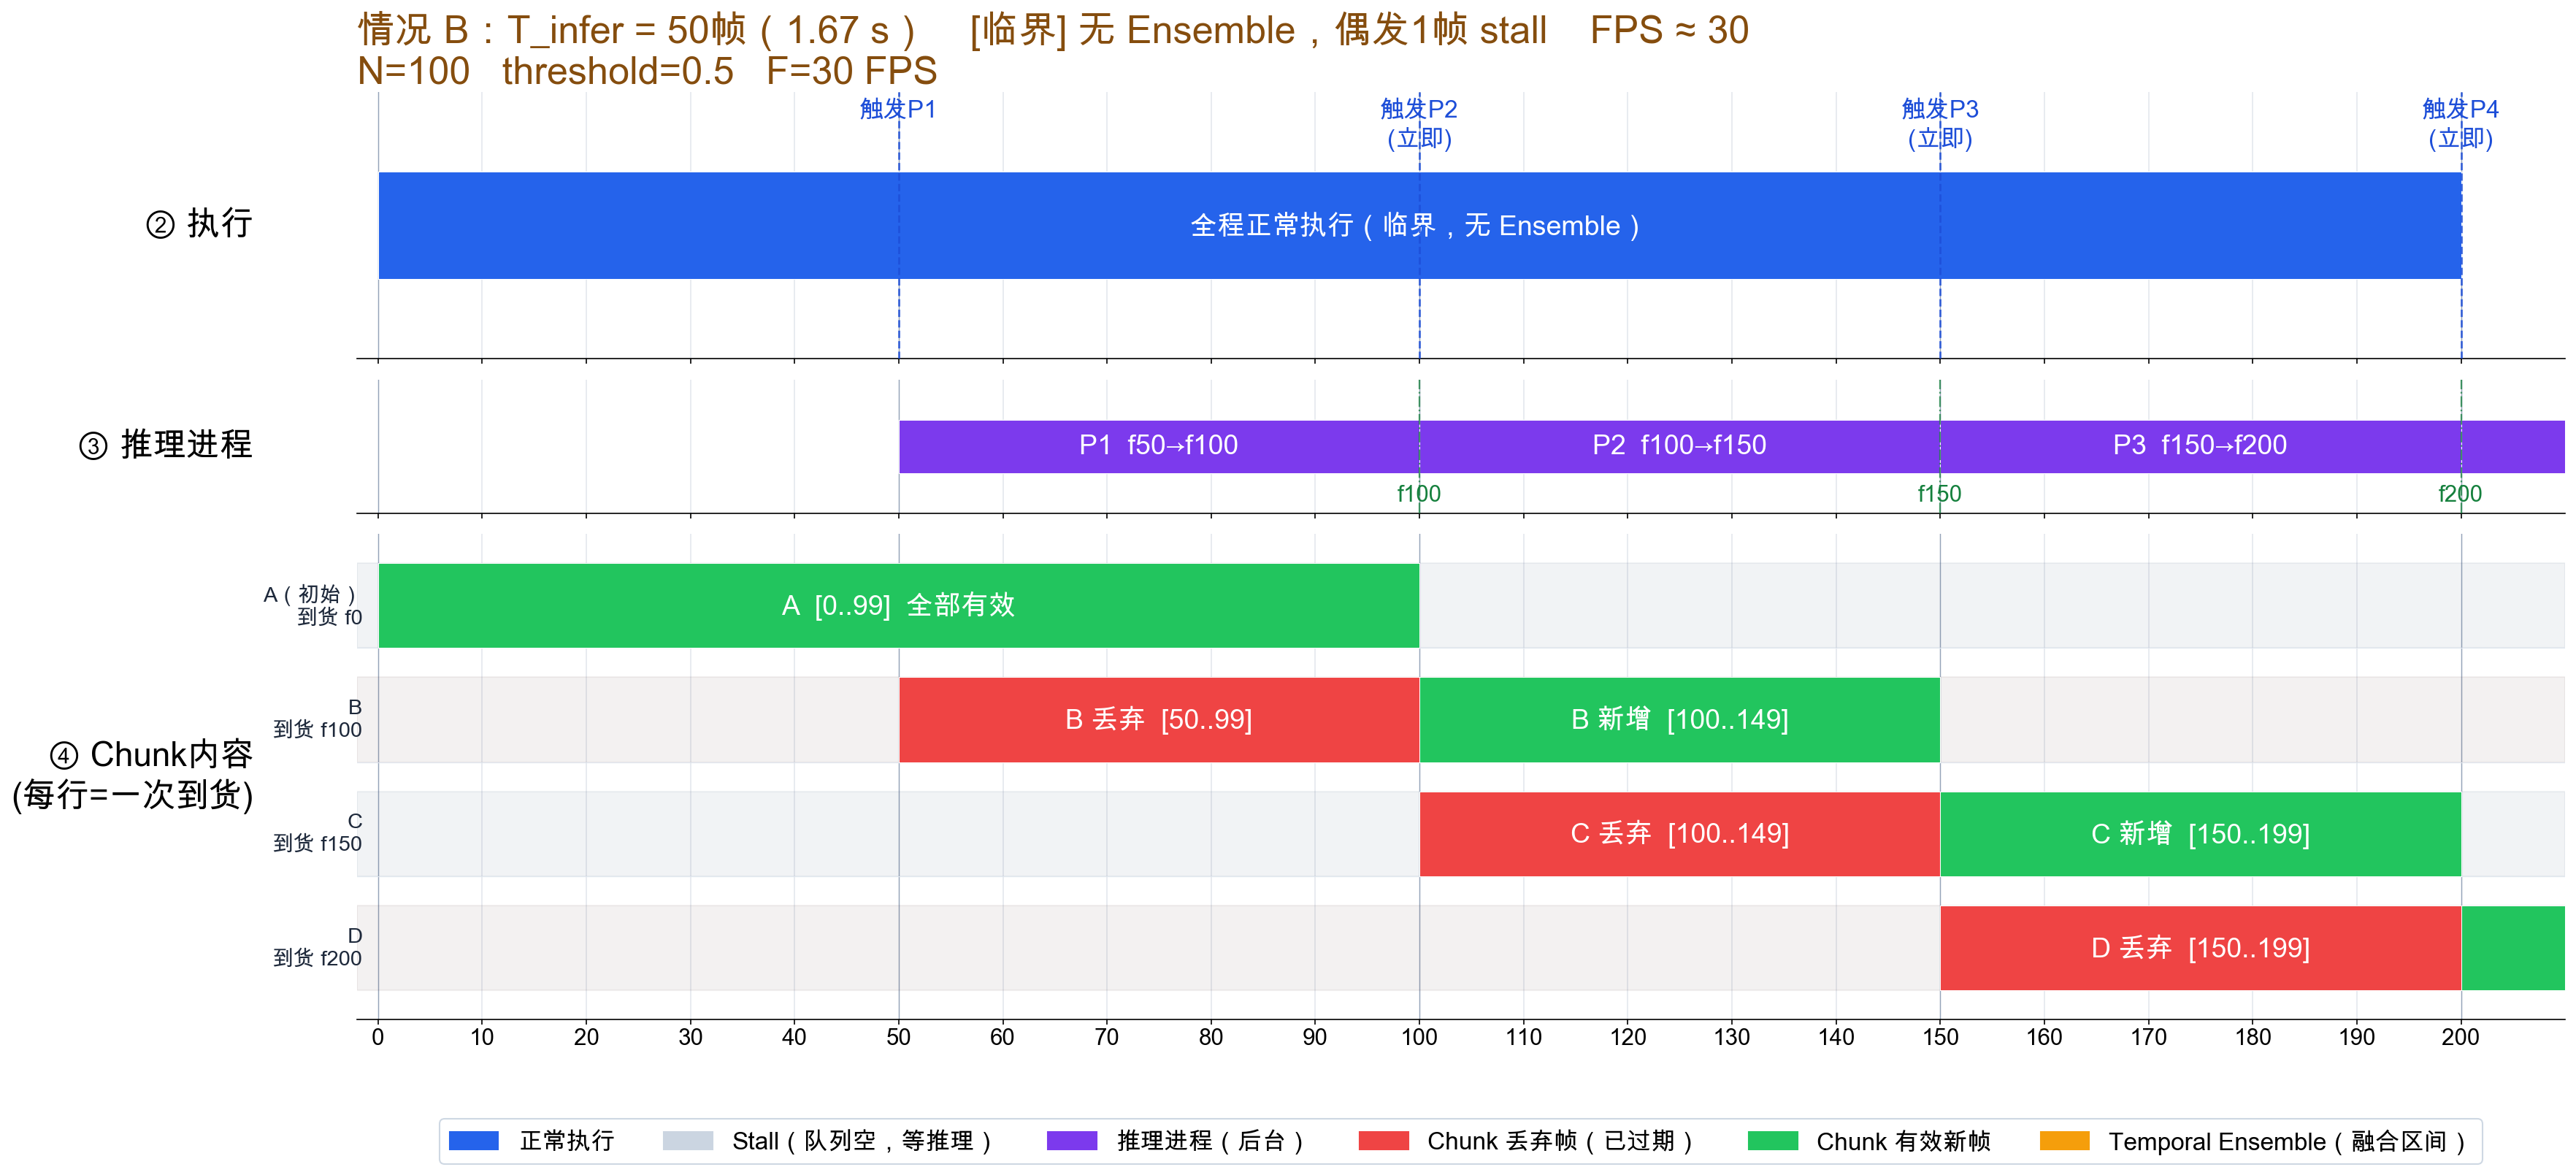
\includegraphics[width=\linewidth]{4_优化/images/async_inference_B.png}
  \caption{情况 B：$T_{\text{infer}}=50$ 帧，恰好处于临界点}
  \label{fig:async-case-b}
\end{figure}

\begin{figure}[htbp]
  \centering
  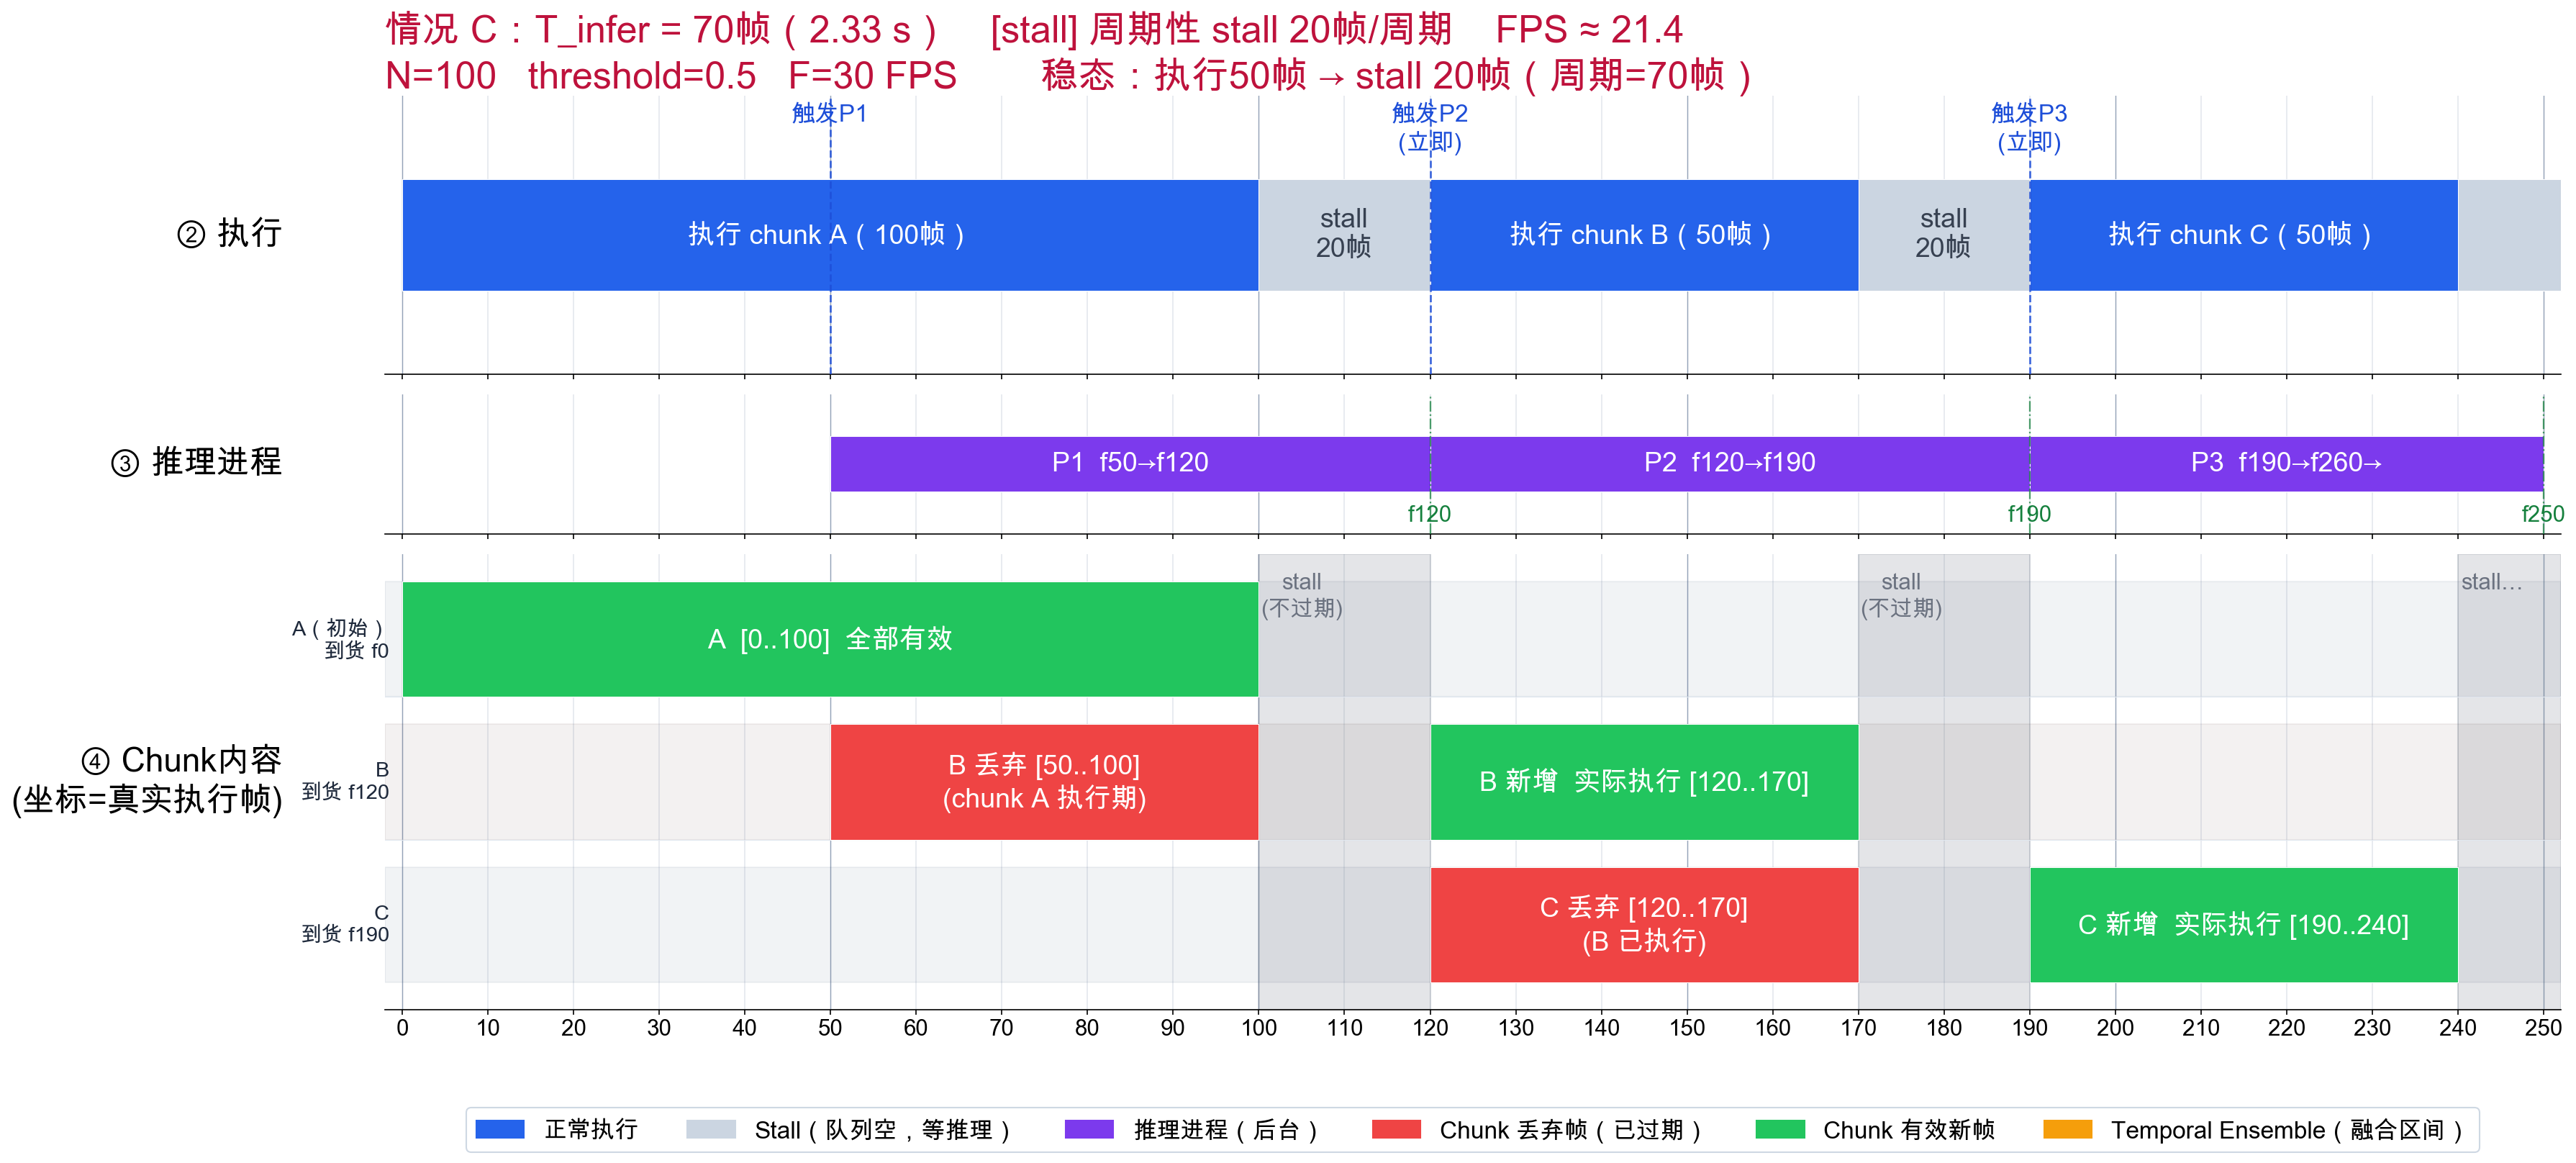
\includegraphics[width=\linewidth]{4_优化/images/async_inference_C.png}
  \caption{情况 C：$T_{\text{infer}}=70$ 帧，不等式不满足，出现周期性 stall}
  \label{fig:async-inf-three-cases}
\end{figure}

值得指出的是情况 C 下的一个微妙之处：stall 期间机器人停止执行，
最新已执行动作步号被冻结，因此当新动作块到货时，
“过期帧”的判定基准并不是“物理时刻已经走过的帧数” $T_{\text{infer}} \cdot F$，
而是 stall 之前最后一次执行到的帧号。
也就是说，stall 的那段时间“反过来保护”了新 chunk 的有效帧不被丢弃。
具体到情况 C，新 chunk 时间戳 $[50, 149]$ 到货时
最新已执行动作步号为 99（chunk A 最末帧），
有效帧数 = $|[100, 149]|$ = 50 而非 30。
这一点必须在公式推导中保留，否则时间线与公式会出现不自洽。

\subsection{平台参数代入}\label{sec:async-inf-substitute}

代入第三章的实测参数 $T_{\text{infer}}$ = 2 s、$F$ = 30 FPS，
可得式（\ref{eq:async-d-substitute}）：
\begin{equation}
  D = T_{\text{infer}}F = 2 \times 30 = 60.
  \label{eq:async-d-substitute}
\end{equation}
在默认 $h=0.5$、$N=100$ 时，边界项如式（\ref{eq:async-bound-substitute}）所示：
\begin{equation}
  \min(hN,\;N/2)=\min(50,\;50)=50 < D,
  \label{eq:async-bound-substitute}
\end{equation}
因此异步流水线无法达到完全无 stall 的 30 FPS 稳态。

需要注意的是，不能在 stall 场景下继续使用
$N_{\text{eff}}=N-D$ 来估算有效 FPS。队列耗尽后机器人停止执行，
最新已执行动作步号不再随物理时间前进，所以返回动作块的过期部分
不会继续扩大。对默认 $h=0.5$ 而言，进入周期性 stall 后，
每轮返回大约仍有 $N/2=50$ 帧可执行；
理想化有效 FPS 近似如式（\ref{eq:async-actual-fps}）所示：
\begin{equation}
  F_{\text{actual}} \;\approx\; \frac{N/2}{T_{\text{infer}}}
  \;=\; \frac{50}{2} \;=\; 25\ \text{FPS},
  \label{eq:async-actual-fps}
\end{equation}
这与后文异步实验中 25 FPS 左右的有效控制频率处在同一量级，
也明显高于同步模式的实测约 16--19 FPS。

从异步推理触发阈值扫描的角度看，更关键的是找到实际临界点：
当异步推理触发阈值小于临界值时，触发太晚，stall 周期性出现；
当异步推理触发阈值越过临界值后，新 chunk 能在旧队列耗尽前到达，
理想稳态就应恢复到 30 FPS。
因此问题从“异步推理是否可用”进一步细化为：
在动作质量仍可接受的前提下，实际临界异步推理触发阈值在哪里，
以及推理本体还需降到多快才能给该临界点留下足够余量。
4.3 节即围绕该参数展开实验扫描。

需要指出的是，上述不等式是在“每次触发都会立即启动一次新推理”的理想假设下推导的。
在 LeRobot 的实际实现中，推理服务进程还会对观测做帧号去重和相似性过滤；
同时，控制端进程、推理服务进程、相机线程和串口通信在树莓派 5
上竞争同一组 CPU 核心。因此，实验中真正起作用的不是纯粹的模型前向耗时，
而是从触发观测到新动作 chunk 合并进队列的有效返回时延。
下文用 $T_{\text{rt}}$ 表示这一端到端有效返回时延，
即从 client 触发观测、server 完成推理，到新动作 chunk 合并入队的实际耗时，
再用 4.3 节的实测数据确定实际临界点。

\subsection{FPS 与异步推理触发阈值的定量关系}\label{sec:async-inf-fps-hold}

4.2.3 节的不等式只给出了稳定无 stall 的边界，却没有回答一个更具体的问题：
在到达该边界之前，也就是确定会发生 stall 的前段区间，
有效 FPS 应该如何随异步推理触发阈值变化？
为避免把代码实现中的抖动误写成理论规律，本节只分析理想调度下的主导关系：
临界点之前 FPS 随异步推理触发阈值上升，临界点之后饱和到目标帧率 30 FPS。
这里先用 $h_{\text{crit}}$ 表示刚好消除 stall 的临界异步推理触发阈值；
若 $h$ 小于该临界值，触发偏晚，旧动作队列会在新 chunk 返回前耗尽。
以下推导只针对临界点之前的 stall 段，即
$h<h_{\text{crit}}$ 且 $T_{\text{rt}}>hN/F$。
实验中的 $h=0.60$ 仅作为偏早触发的参考点，不纳入该段公式。

注意这里不再把 $T_{\text{rt}}$ 强行解释成“实际执行掉的帧数”：
一旦发生 stall，机器人在推理期间实际最多只会继续执行触发时剩余的 $hN$ 帧，
之后就停住等待。

理想化地看，一个周期里只需要数清三件事：执行了多少帧、计算被隐藏了多少、
剩下多少时间必须 stall。触发发生在队列剩余 $hN$ 帧时，
因此计算期间最多能被旧队列继续执行的时间隐藏
$hN/F$。在本节讨论的前段区间中，返回时延一定更长，
因此这里用 $T_{\text{stall}}(h)$ 表示在触发阈值为 $h$ 时，
旧队列耗尽后系统必须空等新 chunk 的时间，
其计算方式如式（\ref{eq:stall-time}）所示：
\begin{equation}
  T_{\text{stall}}(h)
  =
  T_{\text{rt}}-\frac{hN}{F},
  \qquad h<h_{\text{crit}}.
  \label{eq:stall-time}
\end{equation}

在临界点之前，新 chunk 返回时旧队列已经耗尽，
触发时剩余的 $hN$ 帧也已经执行完毕。
因此新 chunk 前部与旧 chunk 重叠的 $hN$ 帧会被判定为过期，
这里用 $E(h)$ 表示每轮新 chunk 返回后仍可作为未来动作执行的帧数，
其近似值如式（\ref{eq:future-action-frames}）所示：
\begin{equation}
  E(h) = N(1-h),
  \label{eq:future-action-frames}
\end{equation}
这里用 $T_{\text{exec}}(h)$ 表示执行这些有效未来动作所需的正常执行时间，
其计算方式如式（\ref{eq:exec-time}）所示：
\begin{equation}
  T_{\text{exec}}(h) = \frac{E(h)}{F}
  = \frac{N(1-h)}{F}.
  \label{eq:exec-time}
\end{equation}

于是一个理想周期的有效 FPS 直接就是
“执行帧数 /（执行时间 + stall 时间）”，
这里用 $F_{\text{eff}}^{\text{ideal}}(h)$ 表示理想调度下、
给定触发阈值 $h$ 时的有效 FPS，
可写为式（\ref{eq:ideal-effective-fps}）：
\begin{equation}
  \begin{aligned}
  F_{\text{eff}}^{\text{ideal}}(h)
  &=
  \frac{E(h)}{T_{\text{exec}}(h)+T_{\text{stall}}(h)} \\
  &=
  \frac{N(1-h)}
       {T_{\text{rt}}+\dfrac{N(1-2h)}{F}}.
  \end{aligned}
  \label{eq:ideal-effective-fps}
\end{equation}
前文提到的临界异步推理触发阈值 $h_{\text{crit}}$
对应 $T_{\text{stall}}(h)=0$ 的边界，
定义如式（\ref{eq:critical-hold}）所示：
\begin{equation}
  h_{\text{crit}} = \frac{T_{\text{rt}}F}{N}
  \label{eq:critical-hold}
\end{equation}
此时 $T_{\text{stall}}=0$，有效 FPS 就达到目标值 $F$；
继续增大异步推理触发阈值就离开本节计算的 stall 段。
在理想模型中，临界点之后不再有 stall，有效 FPS 饱和为 30 FPS。

因此，FPS--异步推理触发阈值曲线的理论形态很简单：
临界点前，异步推理触发阈值增大主要是在缩短 stall，FPS 随之上升；
临界点后，stall 被消除，FPS 饱和到 30。
4.3 节中的实验扫描只需要确定实际部署下的 $h_{\text{crit}}$：
若某个异步推理触发阈值之后的稳态阶段几乎不再出现 stall，
则说明它已经越过临界点；若 episode 平均 FPS 仍低于 30 FPS，
应优先从启动阶段 stall、CPU 资源竞争和调度抖动解释，
而不是把它理解为理论曲线在临界点后的必然下降。

\subsection{树莓派 5 单机部署的 CPU 影响}\label{sec:async-inf-cpu-contention}

异步推理在理论分析之外还有一项需要说明的实际因素：树莓派 5 只有 4 个
ARM Cortex-A76 核心，而模型推理、控制循环、串口通信和相机处理都在同一台设备上运行。
因此，当推理服务进程与控制端进程同机部署时，
两者不可避免地会发生 CPU 资源竞争，进而抬高实际推理耗时。

本章实验并未额外采用绑核或线程数限制等隔离手段，
因此 4.3 节测得的 $T_{\text{infer}}$、有效 FPS 和停顿频次，
都已经包含了这种单机资源竞争带来的影响。
换言之，后文实验结果反映的是当前部署方式下的真实运行表现，
而不是理想隔离条件下的上界性能。
